\section{What's Git?}

%%================================================================================
%%
\subsection{How does Git work?}
%%
%%================================================================================

\begin{frame}
    \frametitle{\secname: \small\subsecname\normalsize}

    \begin{itemize}
        \item Distributed VCS
        \item Initially made as Linux's VCS, to handle and manage large repositories
        \begin{itemize}
            \item In version 5.13 there were:
            \begin{itemize}
                \item 16,306 new commits
                \item ~800,000 lines changed
                \item Involvement of more than 2,000 developers
            \end{itemize}
        \end{itemize}
        \item Each commit represent a new version of the project
        \item A version is a snapshot of the entire repository
    \end{itemize}

    Losing information is really hard! (more on this later)
\end{frame}

%%================================================================================
%%
\subsection{Naming versions}
%%
%%================================================================================

\begin{frame}
    \frametitle{\secname: \small\subsecname\normalsize}

    When you commit a new version to your local repository, Git assigns an identifier to it.

    % git log --decorate=short --decorate-refs-exclude='refs/remotes/*' --decorate-refs-exclude='refs/tags/*' --date-order  --graph --abbrev-commit  --date=short --pretty='format:%C(auto)%d %h (%cd) %s'
    \begin{figure}[h]
        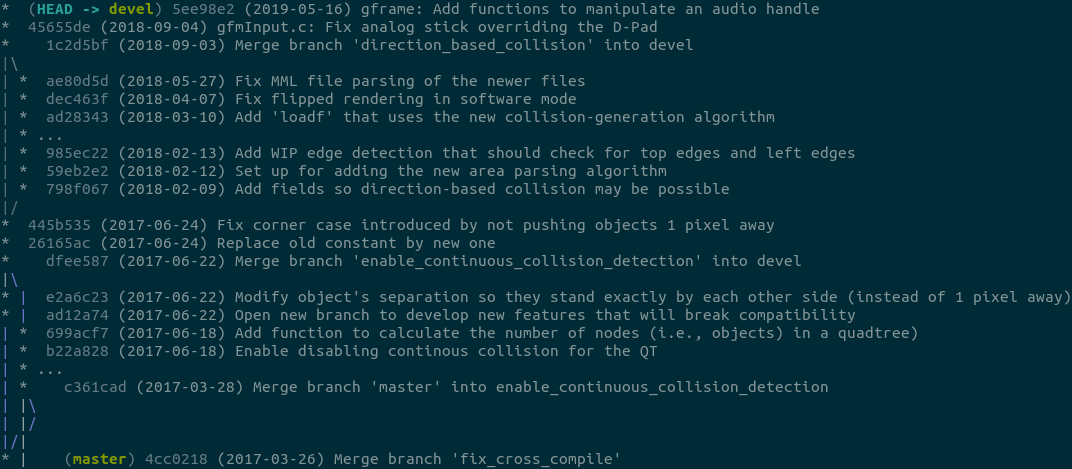
\includegraphics[width=\textwidth]{001-git-commits-example}
        \centering
    \end{figure}
\end{frame}

%%================================================================================
%%
\subsection{Identifying versions}
%%
%%================================================================================

\begin{frame}
    \frametitle{\secname: \small\subsecname\normalsize}

    There are two options to easily track these identifiers:

    \begin{columns}
        % Left side
        \column{0.35\textwidth}

        \begin{figure}[h]
            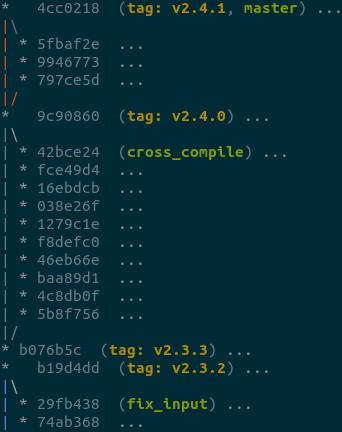
\includegraphics[width=\textwidth]{001-git-branches-example}
            \centering
        \end{figure}

        % Right side
        \column{0.65\textwidth}

        % git log --decorate=short --decorate-refs-exclude='refs/remotes/*' --date-order  --graph --abbrev-commit  --date=short --pretty='format:%C(auto)%h %d ...' master
        \begin{itemize}
            \item \textbf{Tags}: An immutable references to a specific version
            \item \textbf{Branches}: A mutable reference to a version
        \end{itemize}
    \end{columns}

    % XXX: \\ Can't be used as there's no line before this one to be ended
    % (since the last command was a 'column' context).
    \vspace{\baselineskip}
    In both cases, the reference should be meaningfully identified!
\end{frame}

\begin{frame}
    \frametitle{\secname: \small\subsecname\normalsize}

    \textit{HEAD} is a special reference used by Git to identify what's currently checked out in the workspace.

    \begin{figure}[h]
        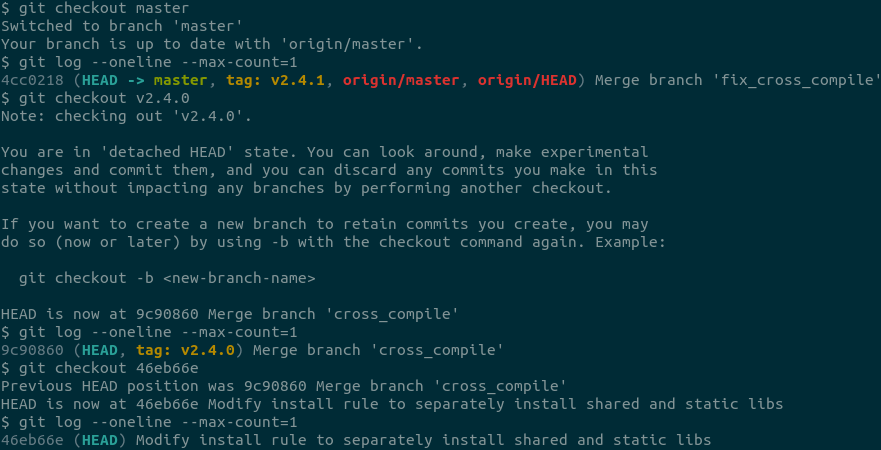
\includegraphics[width=0.8\textwidth]{001-git-checkout-example}
        \centering
    \end{figure}

    \begin{alertblock}{NOTE}
        If Git says something like \textit{You are in 'detached HEAD' state.}, then \textit{HEAD} isn't referencing any branch at all!
    \end{alertblock}
\end{frame}

%%================================================================================
%%
\subsection{"Public" infrastructure vs "Private" infrastructure}
%%
%%================================================================================

\begin{frame}
    \frametitle{\secname: \small\subsecname\normalsize}

    From my personal experience:

    \begin{itemize}
        \item \textbf{Public project}: Changes are made to private copies and later merged back into the original repository
        \item \textbf{Private project}: Changes are made directly to a unique remote copy of the repository
    \end{itemize}

    \begin{columns}
        % Left side
        \column{0.5\textwidth}
        \begin{figure}[h]
            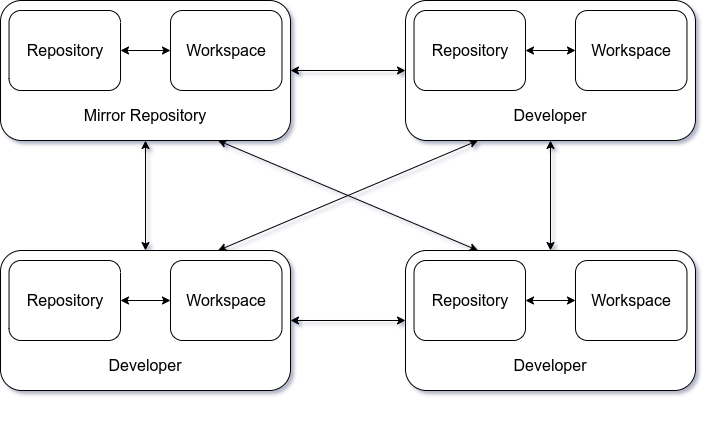
\includegraphics[width=0.95\textwidth]{000-vcs-distributed-plain}
            \centering
        \end{figure}

        % Right side
        \column{0.5\textwidth}
        \begin{figure}[h]
            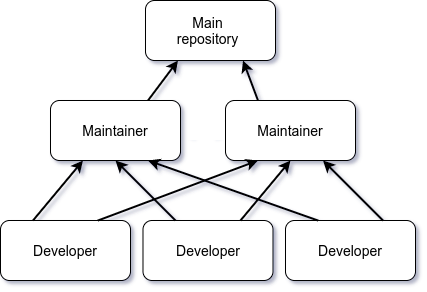
\includegraphics[width=0.95\textwidth]{000-vcs-distributed-hierarchy}
            \centering
        \end{figure}
    \end{columns}
\end{frame}

\begin{frame}
    \frametitle{\secname: \small\subsecname\normalsize}

    Public project example: Linux kernel

    \textit{BASE\_URL}: \small https://git.kernel.org/pub/scm/linux/kernel/git/ \normalsize

    \begin{columns}
        % Left side
        \column{0.35\textwidth}
        \begin{figure}[h]
            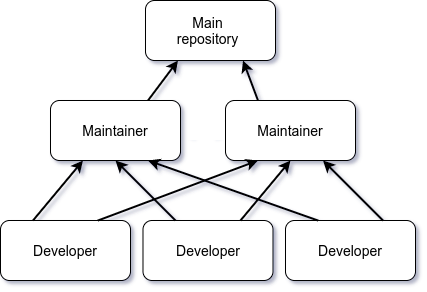
\includegraphics[width=0.95\textwidth]{000-vcs-distributed-hierarchy}
            \centering
        \end{figure}

        % Right side
        \column{0.65\textwidth}
        \begin{itemize}
            \item \textbf{Main repo}: Linus Torvalds' Linux repository
            \begin{itemize}
                \item \small \textit{BASE\_URL}/torvalds/linux.git \normalsize
            \end{itemize}
            \item \textbf{Maintainer}: Staging driver subsystem:
            \begin{itemize}
                \item \small \textit{BASE\_URL}/gregkh/staging.git \normalsize
            \end{itemize}
            \item \textbf{Maintainer}: Media subsystem:
            \begin{itemize}
                \item \small \textit{BASE\_URL}/mchehab/linux-media.git \normalsize
            \end{itemize}
            \item Etc.
        \end{itemize}
    \end{columns}
\end{frame}

%%================================================================================
%%
\subsection{Repository's state}\label{repo-state}
%%
%%================================================================================

\begin{frame}
    \frametitle{\secname: \small\subsecname\normalsize}

    A Git project has three main sections:

    \begin{itemize}
        \item \textbf{Git directory}: Your local copy of the entire repository
        \begin{itemize}
            \item Downloaded when you \textit{clone} a repository from any remote source
        \end{itemize}
        \item \textbf{Working tree}: A single \textit{checkout} of one version of the project, taken from the Git directory
        \begin{itemize}
            \item Basically, everything tracked by Git in the \textit{workspace}
            \item There may be files in the \textit{workspace} that Git isn't tracking
            \item A \textit{bare} copy of a repository is a copy without the \textit{Working tree}
        \end{itemize}
        \item \textbf{Staging area}: changes are marked to go into your next commit
        \begin{itemize}
            \item Stored in the \textit{Git directory}
            \item Relevant enough to deserve its own mention
        \end{itemize}
    \end{itemize}
\end{frame}

\begin{frame}
    \frametitle{\secname: \small\subsecname\normalsize}

    Files in your workspace may be in one of two states:

    \begin{itemize}
        \item \textbf{Tracked}: The file was in the last snapshot, or was staged to be added to the next snapshot
        \item \textbf{Untracked}: The file wasn't in the last snapshot
    \end{itemize}

    Git can't display changes in \textit{untracked}  files since, as far as Git is concerned, those files are brand new.
\end{frame}

\begin{frame}
    \frametitle{\secname: \small\subsecname\normalsize}

    Git has three main states that your files can reside in:

    \begin{itemize}
        \item \textbf{Modified}: The file has changes, either when compared to the latest commit or to the Staging area
        \item \textbf{Staged}: This specific version of the file is marked to be part of the next version
        \item \textbf{Committed}: The data is safely stored in the Git directory
        \begin{itemize}
            \item Could also be called \textit{Unmodified}
        \end{itemize}
    \end{itemize}

    \begin{alertblock}{NOTE}
        These states are exclusively related to the local repository! They don't mean anything in regards to the remote repository!
    \end{alertblock}
\end{frame}

\begin{frame}
    \frametitle{\secname: \small\subsecname\normalsize}

    A file may be both \textit{Modified} and \textit{Staged}, if it was modified after being staged (or if it was only partially staged).

    \begin{figure}[h]
        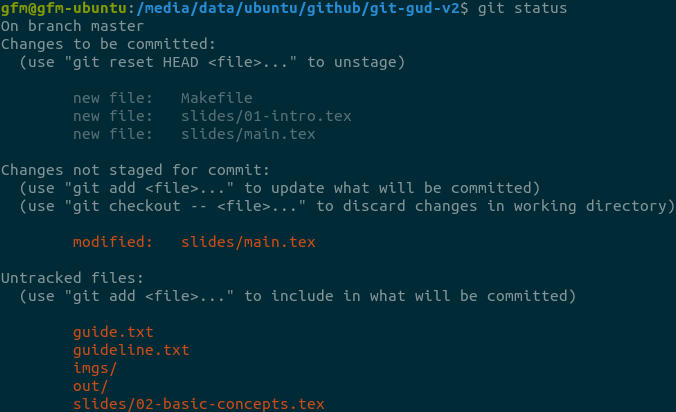
\includegraphics[width=0.9\textwidth]{001-git-areas}
        \centering
    \end{figure}
\end{frame}

%%================================================================================
%%
\subsection{Making changes}
%%
%%================================================================================

\begin{frame}
    \frametitle{\secname: \small\subsecname\normalsize}

    Git creates a snapshot of the entire repository when it creates a new version (commit).

    However, it's OK to think of commits as "changes since the last commit".

    \begin{figure}[h]
        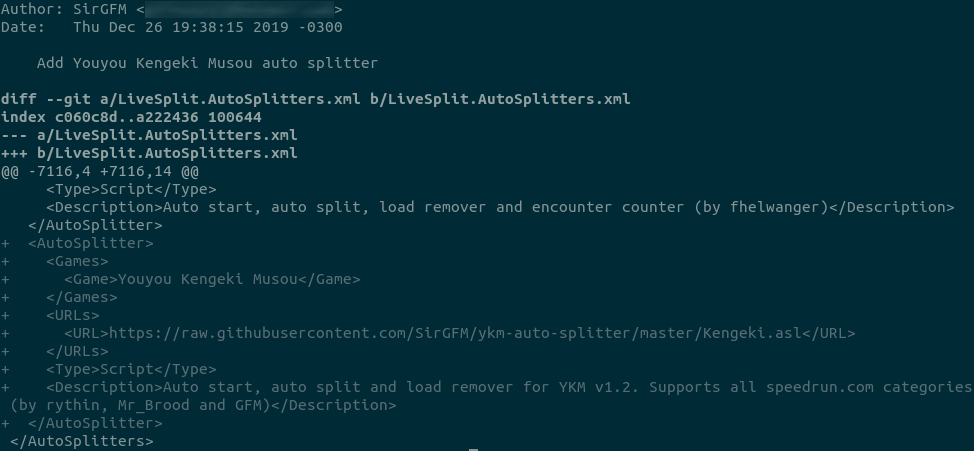
\includegraphics[width=0.95\textwidth]{001-git-diff}
        \centering
    \end{figure}
\end{frame}

%%================================================================================
%%
\subsection{Remote repositories}
%%
%%================================================================================

\begin{frame}
    \frametitle{\secname: \small\subsecname\normalsize}

    Although most operations are done locally, Git is also able to interact with external repositories, called \textit{Remotes}.

    \begin{columns}
        % Left side
        \column{0.5\textwidth}
        \begin{figure}[h]
            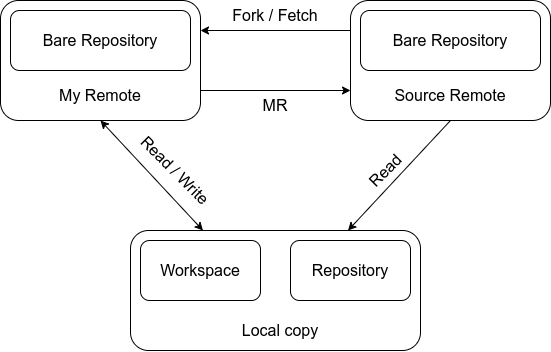
\includegraphics[width=0.95\textwidth]{001-git-remote}
            \centering
        \end{figure}

        % Right side
        \column{0.5\textwidth}
        \begin{figure}[h]
            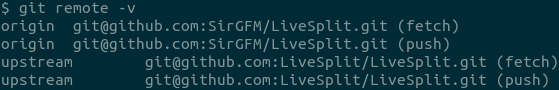
\includegraphics[width=0.95\textwidth]{001-git-remote-example}
            \centering
        \end{figure}
    \end{columns}
\end{frame}

%%================================================================================
%%
\subsection{Integrating changes}
%%
%%================================================================================

\begin{frame}
    \frametitle{\secname: \small\subsecname\normalsize}

    Git repository management services provide means to request that changes made to a given repository/branch are merged into another repository/branch.

    \begin{itemize}
        \item \textbf{Github}: Pull Request
        \item \textbf{Gitlab}: Merge Request
    \end{itemize}

    \begin{figure}[h]
        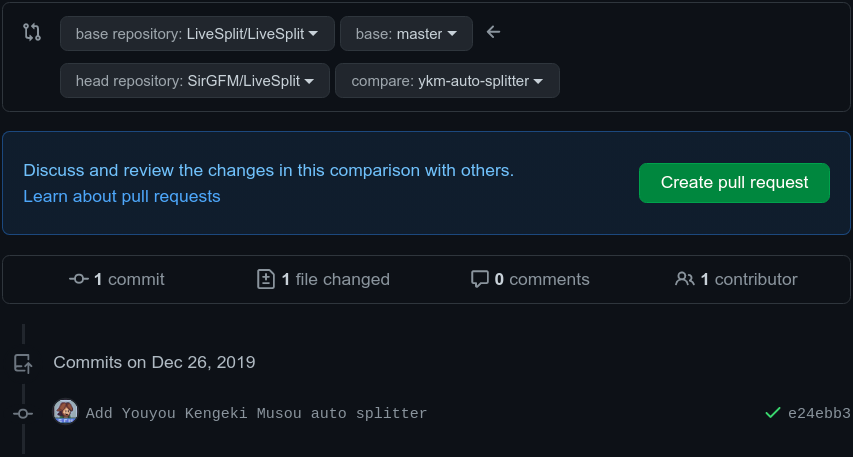
\includegraphics[width=0.8\textwidth]{001-github-mr}
        \centering
    \end{figure}
\end{frame}

\begin{frame}
    \frametitle{\secname: \small\subsecname\normalsize}

    What about repositories outside of one of these services? \\~\\

    For example, how are changes merged back into the Linux kernel?

    \begin{itemize}
        \item Thousands of repositories
        \item Repositories stored in various services/domains
        \item Even local/"offline" repositories
    \end{itemize}
\end{frame}

\begin{frame}
    \frametitle{\secname: \small\subsecname\normalsize}

    \begin{figure}[h]
        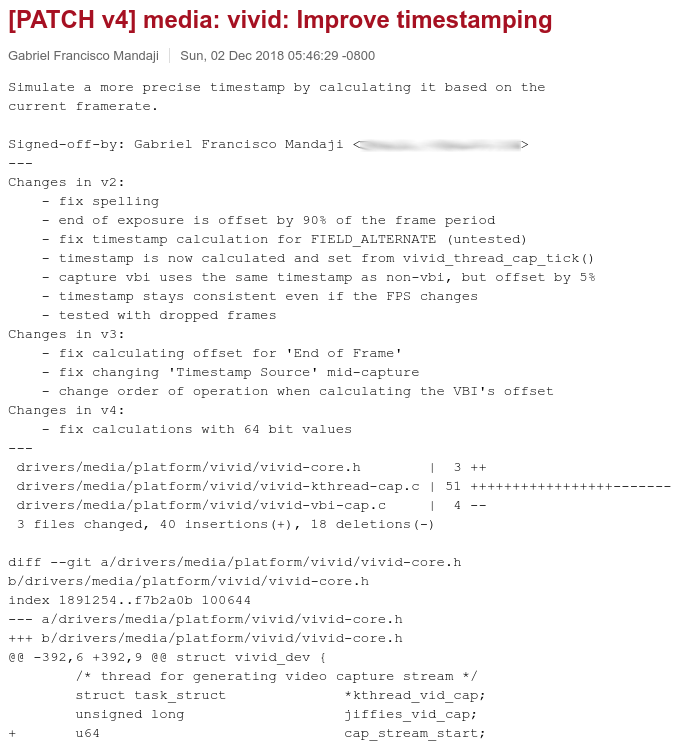
\includegraphics[height=0.8\textheight]{001-linux-mr}
        \centering
    \end{figure}

    Answer: e-mail
\end{frame}
